
%---------------------- % % % Personnalisation des couleurs % % % ----------- BLEU --------
\definecolor{couleurFonce}{RGB}{0,92,133} % Couleur du Code APOGEE
\definecolor{couleurClaire}{RGB}{100,151,186} % Couleur du fond de la bande
\definecolor{couleurTexte}{RGB}{255,255,255} % Couleur du texte de la bande
%------------------------------------------------------------------------------------------



%==========================================================================================
% Semestre 1
%==========================================================================================
\module[codeApogee={UE 11}, 
titre={Algorithmique et programmation 1}, 
CODEUE={2}, 
COURS={}, 
TD={}, 
TP={15}, 
CTD={45}, 
TOTAL={60}, 
SEMESTRE={Semestre 1}, 
COEFF={6}, 
ECTS={6}, 
MethodeEval={Contrôle continue et terminal}, 
ModalitesCCSemestreUn={CC et CT}, 
ModalitesCCSemestreDeux={CT}, 
%CalculNFSessionUne={$\frac{(CC+2*CT)}{3}$}, 
%CalculNFSessionDeux={CT}, 
NoteEliminatoire={}, 
nomPremierResp={Alexandre TESSIER}, 
emailPremierResp={Alexandre.TESSIER@univ-orleans.fr}, 
nomSecondResp={}, 
emailSecondResp={}, 
langue={Français}, 
nbPrerequis={0}, 
descriptionCourte={true}, 
descriptionLongue={true}, 
objectifs={true}, 
ressources={true}, 
bibliographie={false}] 
{
Unité obligatoire. 
}
{
Algorithmique élémentaire\,: expressions, variables, instructions, séquences, conditionnelles, boucles, tableaux, preuves, invariants, traduction dans un langage de programmation orienté objets.
} 
{} 
{\begin{itemize} 
 \ObjItem Maîtriser les concepts élémentaires de l\'algorithmique et être capable de les traduire dans un langages de programmation orienté objets. 
\end{itemize} 
} 
{Ressources} 
{Biblio} 
 
\vfill

%==========================================================================================
\module[codeApogee={UE 12}, 
titre={Atelier de l\'informaticien 1}, 
CODEUE={3}, 
COURS={}, 
TD={}, 
TP={}, 
CTD={24}, 
TOTAL={24}, 
SEMESTRE={Semestre 1}, 
COEFF={3}, 
ECTS={3}, 
MethodeEval={Contrôle continue et terminal}, 
ModalitesCCSemestreUn={CC et CT}, 
ModalitesCCSemestreDeux={CT}, 
%CalculNFSessionUne={$\frac{(CC+2*CT)}{3}$}, 
%CalculNFSessionDeux={CT}, 
NoteEliminatoire={}, 
nomPremierResp={Pierre RETY}, 
emailPremierResp={Pierre.RETY@univ-orleans.fr}, 
nomSecondResp={}, 
emailSecondResp={}, 
langue={Français}, 
nbPrerequis={0}, 
descriptionCourte={true}, 
descriptionLongue={true}, 
objectifs={true}, 
ressources={true}, 
bibliographie={false}] 
{
Unité obligatoire. 
} 
{
Présenter le système sous l\'angle de l\'utilisateur. Configuration de l\'environnement de travail de l\'informaticien 
} 
{} 
{\begin{itemize} 
 \ObjItem Être autonome dans la manipulation du système. 
\end{itemize} 
} 
{Ressources} 
{Biblio} 
 
\vfill

%==========================================================================================
\module[codeApogee={UE 13}, 
titre={Introduction au raisonnement mathématiques}, 
CODEUE={4}, 
COURS={}, 
TD={}, 
TP={}, 
CTD={60}, 
TOTAL={60}, 
SEMESTRE={Semestre 1}, 
COEFF={6}, 
ECTS={6}, 
MethodeEval={Contrôle continue et terminal}, 
ModalitesCCSemestreUn={CC et CT}, 
ModalitesCCSemestreDeux={CT}, 
%CalculNFSessionUne={$\frac{(CC+2*CT)}{3}$}, 
%CalculNFSessionDeux={CT}, 
NoteEliminatoire={}, 
nomPremierResp={François JAMES}, 
emailPremierResp={Francois.JAMES@univ-orleans.fr}, 
nomSecondResp={}, 
emailSecondResp={}, 
langue={Français}, 
nbPrerequis={0}, 
descriptionCourte={true}, 
descriptionLongue={true}, 
objectifs={true}, 
ressources={true}, 
bibliographie={false}] 
{
Unité obligatoire. 
} 
{
Logique naïve et manipulations ensemblistes. Injections, surjections. Structure d\'ordre, cas des réels, majorant, minorant, notion de borne supérieure. Approximations des réels : Q et D. Suites monotones et suites adjacentes. Structure vectorielle de R2 et R3. Sous-espaces vectoriels. Applications linéaires et matrices. Systèmes linéaires. Produit scalaire, produit vectoriel, produit mixte. 
} 
{} 
{\begin{itemize}
 \ObjItem Savoir mettre en \oe uvre un raisonnement mathématique de base. 
\end{itemize} 
} 
{Ressources} 
{Biblio} 
 
\vfill

%==========================================================================================
\module[codeApogee={UE 14}, 
titre={Suites et fonctions réelles}, 
CODEUE={1}, 
COURS={}, 
TD={}, 
TP={}, 
CTD={60}, 
TOTAL={60}, 
SEMESTRE={Semestre 1}, 
COEFF={6}, 
ECTS={6}, 
MethodeEval={Contrôle continue et terminal}, 
ModalitesCCSemestreUn={CC et CT}, 
ModalitesCCSemestreDeux={CT}, 
%CalculNFSessionUne={$\frac{(CC+2*CT)}{3}$}, 
%CalculNFSessionDeux={CT}, 
NoteEliminatoire={}, 
nomPremierResp={Jean-Philippe ANKER}, 
emailPremierResp={Jean-Philippe.ANKER@univ-orleans.fr}, 
nomSecondResp={}, 
emailSecondResp={}, 
langue={Français}, 
nbPrerequis={0}, 
descriptionCourte={true}, 
descriptionLongue={true}, 
objectifs={true}, 
ressources={true}, 
bibliographie={false}] 
{
Unité obligatoire. 
} 
{
Nombres complexes. Suites et fonctions. Fonctions usuelles. Continuité. Dérivabilité. Convexité. Étude de fonctions. 
} 
{} 
{\begin{itemize}
 \ObjItem Savoir mettre en \oe uvre un raisonnement mathématique de base. 
\end{itemize} 
} 
{Ressources} 
{Biblio} 
 
\vfill

%==========================================================================================
\module[codeApogee={UE 15}, 
titre={Arithmétique}, 
CODEUE={1}, 
COURS={}, 
TD={}, 
TP={}, 
CTD={24}, 
TOTAL={24}, 
SEMESTRE={Semestre 1}, 
COEFF={3}, 
ECTS={3}, 
MethodeEval={Contrôle continue et terminal}, 
ModalitesCCSemestreUn={CC et CT}, 
ModalitesCCSemestreDeux={CT}, 
%CalculNFSessionUne={$\frac{(CC+2*CT)}{3}$}, 
%CalculNFSessionDeux={CT}, 
NoteEliminatoire={}, 
nomPremierResp={Patrick MAHEUX}, 
emailPremierResp={Patrick.MAHEUX@univ-orleans.fr}, 
nomSecondResp={}, 
emailSecondResp={}, 
langue={Français}, 
nbPrerequis={0}, 
descriptionCourte={true}, 
descriptionLongue={true}, 
objectifs={true}, 
ressources={true}, 
bibliographie={false}] 
{
Unité obligatoire. 
} 
{
Divisibilité, théorèmes de Bézout et Gauss, décomposition en facteurs premiers. Exemples de structures : anneaux, corps. Congruences, structure de Z/nZ. Aperçu de ces notions dans le cadre de l\'anneau des fonctions polynômes.
} 
{} 
{\begin{itemize}
 \ObjItem Grâce aux exemples d\'arithmétiques élémentaires, découvrir l\'importance de quelques structures algébriques. 
\end{itemize} 
} 
{Ressources} 
{Biblio} 
 
\vfill

%==========================================================================================
\module[codeApogee={UE 16}, 
titre={Anglais 1}, 
CODEUE={1}, 
COURS={}, 
TD={25}, 
TP={}, 
CTD={}, 
TOTAL={25}, 
SEMESTRE={Semestre 1}, 
COEFF={3}, 
ECTS={3}, 
MethodeEval={Contrôle continue et terminal}, 
ModalitesCCSemestreUn={Contrôle continu}, 
ModalitesCCSemestreDeux={Contrôle terminal}, 
%CalculNFSessionUne={$\frac{(CC+2*CT)}{3}$}, 
%CalculNFSessionDeux={CT}, 
NoteEliminatoire={}, 
nomPremierResp={Murielle PASQUET}, 
emailPremierResp={Murielle.PASQUET@univ-orleans.fr}, 
nomSecondResp={}, 
emailSecondResp={}, 
langue={Français}, 
nbPrerequis={1}, 
descriptionCourte={true}, 
descriptionLongue={true}, 
objectifs={true}, 
ressources={true}, 
bibliographie={false}] 
{
Unité obligatoire. 
} 
{
Travail de compréhension et d’expression orale et écrite à partir de documents authentiques simples et/ou courts centrés sur le monde
universitaire anglo-saxon.
} 
{Niveau anglais baccalauréat LV1 ou LV2 ou équivalent.} 
{\begin{itemize} 
 \ObjItem Etre à même de préparer un projet de séjour d’études universitaires en pays anglophone dans une langue écrite et orale simple et suffisamment claire. 
\end{itemize} 
} 
{Ressources} 
{Biblio} 
 
\vfill

%==========================================================================================
\module[codeApogee={UE 17}, 
titre={Préparation au C2I}, 
CODEUE={1}, 
COURS={}, 
TD={24}, 
TP={}, 
CTD={}, 
TOTAL={24}, 
SEMESTRE={Semestre 1}, 
COEFF={3}, 
ECTS={3}, 
MethodeEval={Contrôle continue et terminal}, 
ModalitesCCSemestreUn={CC et CT}, 
ModalitesCCSemestreDeux={CT}, 
%CalculNFSessionUne={$\frac{(CC+2*CT)}{3}$}, 
%CalculNFSessionDeux={CT}, 
NoteEliminatoire={}, 
nomPremierResp={Laure KAHLEM}, 
emailPremierResp={Laure.KAHLEM@univ-orleans.fr}, 
nomSecondResp={}, 
emailSecondResp={}, 
langue={Français}, 
nbPrerequis={0}, 
descriptionCourte={true}, 
descriptionLongue={true}, 
objectifs={true}, 
ressources={true}, 
bibliographie={false}] 
{
Unité obligatoire. 
} 
{
S\'approprier son environnement de travail. Sécuriser son espace de travail local et distant. Pérenniser ses données.
Intégrer les règlementations concernant l\'utilisation des ressources numériques et les règles de bon usage du numérique. Maîtriser son identité numérique.
Maîtriser les fonctionnalités nécessaires à l\'élaboration et la structuration de documents complexes. Traiter des données chiffrées à l\'aide d\'un tableur.
Organiser la recherche d\'informations numériques.
} 
{} 
{\begin{itemize}
 \ObjItem Développer les compétences de base nécessaires à l\'usage des Technologies de l\'Information et de la Communication. 
\end{itemize} 
} 
{Ressources} 
{Biblio} 
 
\vfill


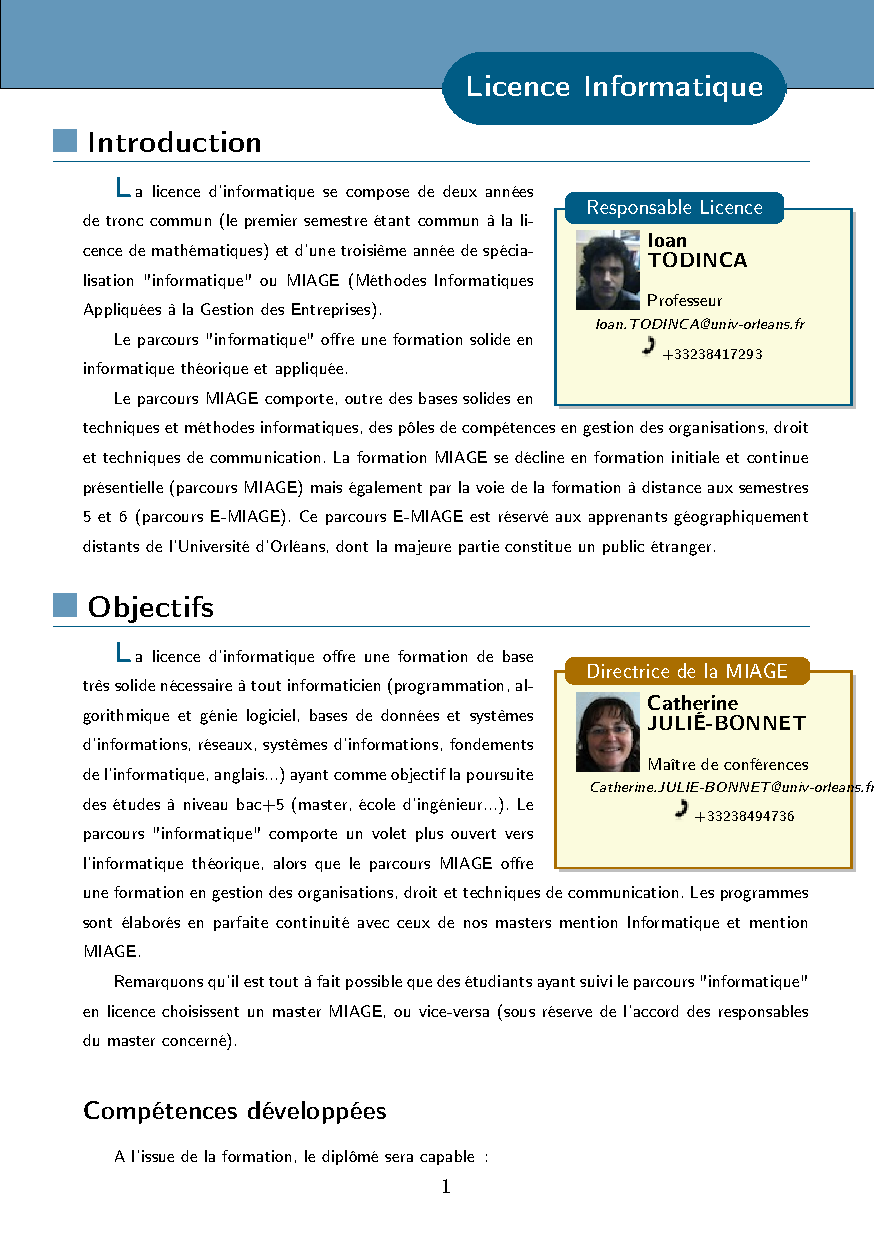
\includepdf[fitpaper,pages=-]{Preambule_Info_LicenceINFO_S2.pdf}

%==========================================================================================
% Semestre 2
%==========================================================================================
\module[codeApogee={UE 21}, 
titre={Algorithmique et programmation 2}, 
CODEUE={1}, 
COURS={}, 
TD={}, 
TP={}, 
CTD={60}, 
TOTAL={60}, 
SEMESTRE={Semestre 2}, 
COEFF={6}, 
ECTS={6}, 
MethodeEval={Contrôle continue et terminal}, 
ModalitesCCSemestreUn={CC et CT}, 
ModalitesCCSemestreDeux={CT}, 
%CalculNFSessionUne={$\frac{(CC+2*CT)}{3}$}, 
%CalculNFSessionDeux={CT}, 
NoteEliminatoire={}, 
nomPremierResp={Wadoud BOUSDIRA}, 
emailPremierResp={Wadoud.BOUSDIRA@univ-orleans.fr}, 
nomSecondResp={}, 
emailSecondResp={}, 
langue={Français}, 
nbPrerequis={1}, 
descriptionCourte={true}, 
descriptionLongue={true}, 
objectifs={true}, 
ressources={true}, 
bibliographie={false}] 
{
Unité obligatoire. 
} 
{
Algorithmique élémentaire\,: récursivité, objets, structures de données chaînées (listes, files, piles), notions élémentaires (allocation dynamique, chaînage des données), traduction dans un langage de programmation orienté objets.
} 
{UE Algorithmique et programmation 1} 
{\begin{itemize}
 \ObjItem Assimiler la programmation récursive d\'une part et d\'autre part, la définition et l\'utilisation de structures de données récursives. 
\end{itemize} 
} 
{Ressources} 
{Biblio} 
 
\vfill

%==========================================================================================
\module[codeApogee={UE 22}, 
titre={Outils mathématiques pour l\'informatique}, 
CODEUE={1}, 
COURS={}, 
TD={}, 
TP={}, 
CTD={50}, 
TOTAL={50}, 
SEMESTRE={Semestre 2}, 
COEFF={6}, 
ECTS={6}, 
MethodeEval={Contrôle continue et terminal}, 
ModalitesCCSemestreUn={CC et CT}, 
ModalitesCCSemestreDeux={CT}, 
%CalculNFSessionUne={$\frac{(CC+2*CT)}{3}$}, 
%CalculNFSessionDeux={CT}, 
NoteEliminatoire={}, 
nomPremierResp={Pierre RETY}, 
emailPremierResp={Pierre.RETY@univ-orleans.fr}, 
nomSecondResp={}, 
emailSecondResp={}, 
langue={Français}, 
nbPrerequis={1}, 
descriptionCourte={true}, 
descriptionLongue={true}, 
objectifs={true}, 
ressources={true}, 
bibliographie={false}] 
{
Unité obligatoire. 
} 
{
Logique des propositions et des prédicats. Étude des procédés de base des démonstrations mathématiques, sur des notions ensemblistes. Relations binaires, fermeture transitive, relations d\'équivalences, relations d\'ordre partiel. Récurrence forte sur la longueur des mots d\'un langage. Algèbre de Boole. Circuits. 
} 
{Les notions ensemblistes} 
{\begin{itemize}
 \ObjItem Comprendre et savoir écrire des démonstrations de mathématiques sur les ensembles et les relations binaires.
 \ObjItem Comprendre les relations d\'équivalences et les relations d\'ordre partiel.
 \ObjItem Être initié aux récurrences non-élémentaires, afin de pouvoir travailler sur l\'induction en 2ème année
 \ObjItem Être initié aux circuits booléens.
\end{itemize} 
} 
{Ressources} 
{Biblio} 
 
\vfill

%==========================================================================================
\module[codeApogee={UE 23}, 
titre={Modélisation}, 
CODEUE={1}, 
COURS={}, 
TD={}, 
TP={}, 
CTD={24}, 
TOTAL={24}, 
SEMESTRE={Semestre 2}, 
COEFF={3}, 
ECTS={3}, 
MethodeEval={Contrôle continue et terminal}, 
ModalitesCCSemestreUn={CC et CT}, 
ModalitesCCSemestreDeux={CT}, 
%CalculNFSessionUne={$\frac{(CC+2*CT)}{3}$}, 
%CalculNFSessionDeux={CT}, 
NoteEliminatoire={}, 
nomPremierResp={Frédéric LOULERGUE}, 
emailPremierResp={Frédéric.LOULERGUE@univ-orleans.fr}, 
nomSecondResp={}, 
emailSecondResp={}, 
langue={Français}, 
nbPrerequis={0}, 
descriptionCourte={true}, 
descriptionLongue={true}, 
objectifs={true}, 
ressources={true}, 
bibliographie={false}] 
{
Unité obligatoire. 
} 
{
Présentation simplifiée de techniques de modélisation et de leur mise en \oe uvre. 
} 
{} 
{\begin{itemize}
 \ObjItem Première approche des principes de modélisation des problèmes informatique. 
\end{itemize} 
} 
{Ressources} 
{Biblio} 
 
\vfill
